%!TEX root = TQFTnotes.tex
%%%%%%%%%%%%%%
\chapter{Higher categories}\label{c:higher-cat}

In the previous chapters, we have defined extended 2d TQFTs using
the language of weak 2-categories and symmetric monoidal 2-categories. In a
similar way, it is clear that to define extended TQFTs in higher
dimensions, we will need higher categories: if we have a good definition of
an $n$-category, and we can construct the category of cobordisms with
corners $\Bord_n$, we can define an extended $n$-dimensional TQFT as a
symmetric monoidal functor $\Bord_n\to \calC$, for some symmetric monoidal
$n$-category $\calC$.

In this chapter, we discuss various approaches to defining higher categories. We
will restrict ourselves to a very brief overview, referring the reader to
original papers for details.




%%%%%%%%%%%%%%%%
\section{Fundamental groupoid}\label{s:fundamental-groupoid}

Reversing the traditional order in mathematics, we begin our discussion of
higher categories not with a definition but with an example: whatever definition
we give later, it should cover that example. This example is that of a
fundamental groupoid, described informally below.


Recall that for a topological space $X$, we denote by $\Pi(X)$ the fundamental
groupoid of $X$; it is a category whose objects are points of $X$ and morphisms
are homotopy classes of paths in $X$.

We can extend it and define the fundamental infinity groupoid $\Pi_{\infty}(X)$
as follows:
\begin{itemize}
  \item Objects of $\Pi_{\infty}(X)$ are points of $X$.
  \item 1-morphisms $x_0\to x_1$ are paths in $X$, i.e., continuous maps
    $I\to X$ such that $\ga(0)=x_0$, $\ga(1)=x_1$ (here and below, $I=[0,1]$).
  \item 2-morphisms $\ga_0\to \ga_1$, where $\ga_i$ are paths from $x_0$ to
  $x_1$, are path homotopies, i.e., continuous maps $h\colon I^2\to X$ such that
  $h(0,t)=\ga_0(t)$, $h(1, t)=\ga_1(t)$, and for all $s$, $h(s,0)=x_0$,
  $h(s,1)=x_1$.
  \item 3-morphisms are homotopies between homotopies, i.e., continuous maps
  $I^3\to X$ with suitable restrictions to the boundary.
  \item \dots
\end{itemize}
This defines an ``infinity groupoid'', which has morphisms of all orders. We can
also define the fundamental $n$-groupoid $\Pi_{\leq n}(X)=\tau_{\leq
n}(\Pi_\infty(X))$, which only has morphisms up to order $n$: namely,
$n$-morphisms in $\Pi_{\leq n}(X)$ are homotopy classes of
$n$-morphisms in $\Pi_{\infty}(X)$ (two $n$-morphisms are homotopic if there
exists an $(n+1)$-morphism between them in $\Pi_\infty(X)$).

Note that we have not yet discussed composition in $\Pi_\infty(X)$. It is easy
to define composition in the same way as it is done in the usual fundamental
groupoid $\Pi_{\le 1}(X)$; however, so defined composition is not associative in
$\Pi_\infty$. For example, for $1$-morphisms $\ga_1, \ga_2, \ga_3$, the
compositions $\ga_3 (\ga_2 \ga_1)$ and $(\ga_3 \ga_2)\ga_1$ are not equal as
maps $I\to X$: in the first case, $\ga_1$ is traveled over $t\in [0, 1/4]$,
$\ga_2$ over $t\in [1/4, 1/2]$, and $\ga_3$ over $[1/2,1]$. For the second
composition, the intervals are $[0, 1/2]$, $[1/2, 3/4]$, and $[3/4,1]$
respectively, so these compositions are not equal; however, they are homotopic
to each other. Thus, any definition of an $n$-category should allow for
compositions ``associative up to homotopy''.


Fundamental $n$-groupoids $\Pi_{\leq n}(X)$ were suggested by Grothendieck in
\ocite{grothendieck}. He also proposed the following hypothesis.
\begin{conjecture}[Homotopy hypothesis]
  Homotopy $n$-types up to weak equivalence
  are classified by $\Pi_{\leq n}(X)$ up to equivalence.
\end{conjecture}
(Recall that a topological space $X$ is called an \emph{$n$-type} if its
homotopy groups $\pi_k(X)$ are trivial for $k>n$.)

Of course, in order to discuss this hypothesis, one needs first to give a
definition of $n$-categories and equivalences between them; thus, we should
consider this hypothesis as a natural requirement which should be satisfied by
any definition of an $n$-category.

One can also state an $\infty$ version of the homotopy hypothesis; namely, it
says that topological spaces up to weak equivalence are classified by their
$\infty$ fundamental groupoids up to equivalence.

%%%%%%%%%%%%%%%%
\section{Strict and weak $n$-categories}\label{s:strict-n-cat}
After giving the motivating example of $n$-groupoids, we can try to
define the notion of an $n$-category.

The simplest approach is considering strict $n$-categories. These categories are
not very hard to define. Namely, a strict $n$-category must have objects, and
for any objects $X,Y$, we must have an $(n-1)$-category $\Hom (X,Y)$, together
with a composition functor of $(n-1)$-categories $\Hom(X,Y)\times \Hom(Y,Z)\to
\Hom(X,Z)$, which must be associative. In a similar way one defines identity
morphisms. (Category theorists would say that an
$n$-category is a category enriched over $(n-1)$-categories.)

However, this definition is not of much use. First, virtually all known examples
are non-strict --- compositions are not strictly associative but only
``associative up to higher order isomorphisms'', as we have already seen in the
example of fundamental groupoids. Moreover, for $n\ge 3$, it turns out that this
is more than just a technical problem: not every weak 3-category is equivalent
to a strict 3-category (unlike the case of 2-categories). For example, it can be
shown that $\Pi_{\leq 3}(S^2)$, the truncated fundamental
groupoid of $S^2$, is not equivalent to a strict 3-groupoid (see
\ocite{simpson}*{Theorem 2.7.2}).



Thus, we have no choice but to forget strict categories and start developing the
theory of weak $n$-categories, where compositions are ``associative up to
higher order isomorphisms''.


Unfortunately, giving an algebraic definition of a weak $n$-category is very
hard to do. A definition of a weak 3-category exists (see
\ocite{gordon-power-street}), but it is so long that I was never able to get to
the end of it; for $n\ge 4$, the algebraic definitions are even more cumbersome.
Some summary of algebraic approaches is collected in \ocite{leinster}. On the
other hand, there are a number of rather easy to define examples of (weak) 3-
and 4-categories, some of which we will give later.


%%%%%%%%%%%%%%%%%%%%%%%%%%%%%%%%%%%%%%%%%%%%%%

\section{Weak categories and infinity categories}\label{s:infinity-categories}

An alternative approach to the notion of a weak $n$-category is to use the
ideas of topology, or more precisely, homotopy theory. The key idea of this
approach is that instead of defining a single composition operation which is
weakly associative, we allow many composition operations, which must form a
contractible space. Paths in this contractible space correspond to
$(k+1)$-isomorphisms between the corresponding compositions, homotopies between
paths correspond to $(k+2)$-isomorphisms, etc. Different compositions give
different points in this contractible space; the fact that they are all
isomorphic follows from the fact that this space is connected, and all
compatibility relations between these isomorphisms follow from the fact that the
space of compositions is contractible.

This idea can be used to define weak $n$-categories; it can also be used to
define $(\infty, n)$ categories. Informally, an $(\infty, n)$ category is a
category which has morphisms of all orders $k \ge 1$, but for $k>n$, all
$k$-morphisms are invertible.


Of course, the above is not yet a definition; even for $n=1$, developing this
idea and turning it into a precise definition is non-trivial. In fact, there are
many competing ways to define the notion of $(\infty, 1)$ category, all giving
different formalizations of the above idea. Among them:

\begin{itemize}
  \item Quasicategories, also known as weak Kan complexes
  \item Complete Segal spaces
  \item Segal categories
\end{itemize}

Fortunately, it turns out that in a certain sense all these definitions are
equivalent. There are a number of papers discussing this, including
\ocite{toen}, \ocite{bsp}, and the book \ocite{riehl-verity}; for a short
introduction, there is also Emily Riehl's article \ocite{riehl-notices} in
the Notices of the AMS. We will not be discussing this at all; we will restrict
ourselves to giving just one definition, based on Segal categories. This
construction takes some time; we will do it in the next several sections. Our
exposition follows the paper \ocite{schommer-pries-category}; a detailed exposition of
the theory of Segal categories as a model for $(\infty, n)$ categories can be
found in \ocite{simpson}.



%%%%%%%%%%%%%%%%%
\section{Nerve of a category}\label{s:nerve}
Before giving a definition of a weak category, let us take another look at the
definition of a usual category. Let $\calC$ be a category; define a collection
of sets $X_n$, $n\ge 0$ by
\begin{equation}\label{e:nerve1}
  \begin{aligned}
    X_0&= \Obj \calC \quad (\text{objects of $\calC$})\\
    X_1&= \{ (x_0, x_1, f)\st x_i \in \calC, f\colon x_0\to x_1\}
                \quad (\text{morphisms in $\calC$})\\
                &\dots\\
    X_n&=\{(x_0, \dots, x_n, f_1, \dots, f_n)\st
           x_i \in \calC, f_i\colon x_{i-1}\to x_i \}\\
            &\quad (\text{composable $n$-chains of morphisms in $\calC$})\\
  \end{aligned}
\end{equation}
Then all compositions and units in $\calC$ can be described in terms
of maps between these sets. For example, we have the composition map
\begin{align*}
  X_2&\to X_1\\
  (x_0\xto{f_1} x_1 \xto{f_2}x_2)&\mapsto (x_0\xto{f_2f_1} x_2)
\end{align*}
and a unit map
\begin{align*}
  X_0&\to X_1\\
  x&\mapsto (x\xto{1_x} x)
\end{align*}

More generally, we have \emph{face maps}
\begin{equation}\label{e:nerve2}
  \begin{aligned}
  d_i\colon X_n&\to X_{n-1}, \qquad 0\le i \le n\\
  (\dots x_{i-1}\xto{f_i} x_i \xto{f_{i+1}} x_{i+1}\to \dots)
  &\mapsto
  (\dots x_{i-1}\xto{f_{i+1}f_i} x_{i+1}\to \dots)
  \end{aligned}
\end{equation}
(for $i=0$, this map deletes both object $x_0$ and morphism $f_1$; for $i=n$,
it deletes $x_n$ and $f_n$).

We also have \emph{degeneracy maps}
\begin{equation}\label{e:nerve3}
  \begin{aligned}
  s_i\colon X_n&\to X_{n+1}, \qquad 0\le i \le n\\
  (\dots \xto{f_i} x_i \xto{f_{i+1}} \dots)
  &\mapsto
  (\dots \xto{f_i} x_i \xto{1_{x_i}} x_i \xto{f_{i+1}} \dots)
  \end{aligned}
\end{equation}

One should think of $d_i$ as ``erasing'' the object $x_i$ in the chain, and $s_i$
as doubling $x_i$ and inserting the identity morphism. (The names ``face map''
and ``degeneracy map'' are motivated by the relation to homotopy theory; see
\seref{s:sset}.)

These maps satisfy a number of relations, which follow from (and in fact are
equivalent to) the associativity and unit axioms for the category $\calC$. One can write
these relations explicitly; however, there is a more elegant way to do that,
using the notion of \emph{simplicial set}.\index{simplicial set}

\begin{definition}\label{d:simplex-category}\index{simplex category}
The \emph{simplex category} $\Ddelta$ is the category whose objects are
totally ordered sets $[n] = \{0,1,\dots,n\}$, $n \ge 0$, and morphisms are
(non-strictly) order preserving functions.
\end{definition}
In particular, for each $n\ge 0$, there are $n + 1$ injections
$d^i\colon [n-1] \to [n]$, called the coface maps, and
$n + 1$ surjections $s^i \colon [n + 1] \to [n]$,
called the codegeneracy maps, defined as follows:
$$
d^i(k) = \begin{cases}
            k & \quad k<i\\
            k+1 & \quad k\ge i
          \end{cases}
\qquad \qquad
s^i(k) = \begin{cases}
            k & \quad k\le i\\
            k-1 & \quad k> i
          \end{cases}
$$
The $i$-th coface map $d^i$ misses the element $i$ in the image, while $s^i$
sends two elements to $i$. It is easy to show that these maps generate all
morphisms in $\Ddelta$: any order-preserving map is a composition of coface and
codegeneracy maps.

\begin{definition}\label{d:simplicial-set}
  A simplicial set is a functor $X\colon \Ddelta^\op\to \sets$.
\end{definition}
It is common to use notation $X_n=X([n])$ and $d_i=X(d^i)\colon X_{n}\to
X_{n-1}$, $s_i = X(s^i)\colon X_n\to X_{n+1}$.

(Again, the motivation for the name ``simplicial set'' will be given in
\seref{s:sset}.)

It is easy to see that simplicial sets form a category, with morphisms being
morphisms of functors; in other words, given two simplicial sets $X_\bullet$,
$Y_\bullet$, a morphism $f\colon X_\bullet \to Y_\bullet$ is a collection of
maps $f_n\colon X_n\to Y_n$ which commute with all $d_i, s_i$. We denote by
$\ssets$ the category of simplicial sets.

\begin{theorem}\label{t:nerve}
  Let $\calC$ be a category. Then formulas \eqref{e:nerve1}--\eqref{e:nerve3}
  define a simplicial set, called the \emph{nerve} of $\calC$.
  \index{nerve of a category}
\end{theorem}
\begin{exercise}\label{ec:associativity-axiom}
  Write explicitly the associativity axiom in $\calC$ as an equality of two
  maps $X_3\to X_1$, and write the corresponding relation between coface maps
  $d^i$ in $\Ddelta$.
\end{exercise}

One can ask if it is possible to describe which simplicial sets appear
as nerves of categories. To answer that, we recall the notion of fiber
product.

Assume that we have two sets $A_1, A_2$ and maps $p_i\colon A_i\to B$. The
fiber product $A_1\times_B A_2$ is defined by
$$
A_1\times_B A_2 = \{(a_1, a_2)\in A_1\times A_2\st p_1(a_1)=p_2(a_2)\}
$$
Clearly, we have canonical maps $A_1\times_B A_2\to A_i$ which make the
diagram below commutative (this diagram is frequently called the
\emph{pullback square})\index{pullback square}
\begin{equation}\label{e:pullback}
\begin{tikzpicture}[vcenter]
\node (p) at (0,0) {$A_1\times_B A_2$};
\node (a1) at (0, -1.5) {$A_1$};
\node (a2) at (2, 0) {$A_2$};
\node (b) at (2, -1.5) {$B$};
\draw[->] (p)--(a1);
\draw[->] (p)--(a2);
\draw[->] (a1)--(b);
\draw[->] (a2)--(b);
\end{tikzpicture}
\end{equation}

A better definition --- which also works in other situations, for example when
$A_i, B$ are topological spaces and all maps are continuous --- defines
$A_1\times_B A_2$ as the universal object in the category of diagrams: for
every diagram below, there is a unique map $P\to A_1\times_B A_2$
\begin{equation*}
  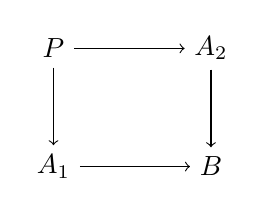
\begin{tikzpicture}
    \node (p) at (0,0) {$P$};
    \node (a1) at (0, -1.5) {$A_1$};
    \node (a2) at (2, 0) {$A_2$};
    \node (b) at (2, -1.5) {$B$};
    \draw[->] (p)--(a1);
    \draw[->] (p)--(a2);
    \draw[->] (a1)--(b);
    \draw[->] (a2)--(b);
  \end{tikzpicture}
\end{equation*}


It is easy to see that for the nerve of a category $\calC$, in other words,
when $X_n$ is given by \eqref{e:nerve1}, we have maps
\begin{align*}
p_i \colon X_n&\to X_1\\
(\dots \to x_{i-1} \xto{f_i} x_i\to \dots )&\mapsto ( x_{i-1} \xto{f_i} x_i).
\end{align*}
Thus, by the universality property of the fiber product, we have the \emph{Segal map}
\index{Segal!map}
\begin{equation}\label{e:segal-map}
   s_n\colon X_n \to
   X_1\times_{X_0} X_1\times_{X_0} X_1 \times\dots \times_{X_0} X_1.
\end{equation}
Maps $p_i$ (and thus, the Segal map $s_n$) can be defined for any simplicial set:
they correspond to the map $[1]\to[n]\colon 0\mapsto (i-1), 1\mapsto i$ in
$\Ddelta$.

\begin{theorem}\label{t:segal1}
  A simplicial set $X$ is a nerve of some category $\calC$ if and only if the
  following \emph{Segal condition}\index{Segal!condition} holds: for every $n\ge
  1$, the Segal map \eqref{e:segal-map} is a bijection
  \begin{equation}\label{e:segal1}
    X_n \simeq X_1\times_{X_0} X_1\times_{X_0} X_1 \times\dots \times_{X_0} X_1.
  \end{equation}
\end{theorem}
The proof of this theorem is straightforward:
it is just another way of saying that any
composable chain of morphisms consists of an $n$-tuple of morphisms where the
target of the $i$-th morphism coincides with the source of the $(i+1)$-st one.


Thus, (usual) categories can be described as simplicial sets satisfying the Segal
condition \eqref{e:segal1}.

%%%%%%%%%%%%%%%%%
\section{Simplicial sets as models of topological spaces}\label{s:sset}

In the previous section, simplicial sets (i.e., functors $\Ddelta^\op\to \sets$)
were introduced as a natural language to describe nerves of categories. However,
historically simplicial sets appeared in topology. In this section, we briefly
review that, referring the reader to the books \ocite{may},
\ocite{goerss-jardine} for details.

Throughout this section, we will denote by $\ssets$ the category of simplicial
sets.

\begin{example}\label{x:top-sset}
  Let $X$ be a topological space. For any $n\ge 0$, define the set
  $\Sing(X)_n$ by
  $$
    \Sing(X)_n= \{\text{continuous maps }\Delta^n\to X\}
  $$
  where $\Delta^n$ is an $n$-dimensional simplex
  \begin{equation}\label{e:simplex}
    \Delta^n=\Bigl\{
              (t_0, t_1, \dots, t_n)\in \R^{n+1}\st
              0\le t_i \le 1, \quad \sum t_i=1
             \Bigr\}.
  \end{equation}
  Vertices of $\Delta^n$ are in natural bijection with $[n]$, and any
  order-preserving map $f\colon [m]\to [n]$ defines an affine linear
  map $f\colon \Delta^m \to \Delta^n$. Precomposition with $f$ defines on
  $\Sing_\bullet$ the structure of a simplicial set.
\end{example}
Thus, we have a functor
$$
  \Sing\colon \Top \to \ssets
$$
usually called the \emph{singular complex}\index{singular complex} of $X$.
Moreover, many usual constructions for topological spaces, such as the notion of
homotopy of maps, or the notion of direct product, can be easily generalized to
simplicial sets. (In fact, it can be shown that for any topological space $X$,
the singular complex $\Sing(X)$ has an additional property, existence of
certain extensions; such simplicial sets are called \emph{Kan complexes}.)

It turns out that we also have a \emph{geometric realization
functor}\index{geometric realization functor} $|\quad|\colon \ssets\to \Top$;
roughly, for a simplicial set $K$ we take the disjoint union of (topological)
simplices, one copy of $\Delta^n$ for each point $x\in K_n$, and then ``glue''
them together using the face maps. Details can be found, e.g., in
\ocite{may}*{Chapter III}. In particular, $|K|$ is always a CW complex.

The functors $\Sing\colon \Top\to \ssets$ and $|\quad|\colon \ssets\to \Top$ are
adjoints of each other: we have a functorial isomorphism
$$
  \Hom_{\ssets}(K, \Sing(X))\simeq \Hom_{\Top}(|K|, X),
  \qquad X\in \Top, K\in \ssets
$$
(\ocite{may}*{\S 15}). The unit and counit of this adjunction, therefore,
give us morphisms
\begin{align*}
  \Psi&\colon K\to \Sing(|K|),\\
  \Phi&\colon |\Sing(X)|\to X.
\end{align*}

The following theorem is well-known (see e.g., \ocite{may}*{\S 16};
\ocite{goerss-jardine}*{Theorem I.11.4}).
\begin{theorem} \label{t:sset-top}
\par\noindent
  \begin{enumerate}
    \item For any simplicial set $K$, $\Psi\colon K\to \Sing(|K|)$ is an
      embedding of simplicial sets, which is a weak homotopy equivalence.
      If $K$ is a Kan complex, then $\Psi$ is a homotopy equivalence.
    \item
      For any topological space $X$, $\Phi\colon |\Sing(X)|\to X$ is surjective
      and is a weak homotopy equivalence. If $X$ is a CW complex, then $\Phi$
      is a homotopy equivalence.
  \end{enumerate}
\end{theorem}

Thus, one can think of simplicial sets as a combinatorial model for the study of
homotopy of topological spaces. In many ways, $\ssets$ is easier to work with
than the category $\Top$; for example, $\ssets$ has a natural structure of a
Quillen closed model category (which we are not going to discuss; interested
readers should check, e.g., \ocite{simpson}*{Section 7} or
\ocite{goerss-jardine}*{Section I.11}).



%%%%%%%%%%%%%%%%%%%%%%%%%%%%
\section{Enriched categories}\label{s:enriched-cat}

In the previous sections, we gave a description of a (usual) category $\calC$ as
a simplicial set satisfying additional Segal condition. In a similar way, one
can describe \emph{enriched categories}, i.e., categories where $\Hom$ spaces
are not just sets, but have additional structure --- e.g., they are topological
spaces. For example, if we denote by $\Top$ the category of topological spaces
with continuous maps, a $\Top$-enriched category is the following data:
\begin{enumerate}
\item A class $S$ of objects of $\calC$
\item For any pair of objects $x,y\in S$, a topological space
  $\Hom(x,y)$
\item For any triple of objects, a continuous map
      $\Hom(x,y)\times \Hom(y,z)\to \Hom(x,z)$
\item For any object $x\in S$, a point $1_x\in \Hom(x,x)$
\end{enumerate}
satisfying the usual (strict) associativity and unit axioms. As usual, we
restrict our attention to small categories, so we assume that objects form a
set.

As before, we can describe such categories using simplicial sets --- or more
generally, simplicial objects in an appropriate category.


\begin{definition}\label{d:simplicial-object}
  Let $\calM$ be a category. A \emph{simplicial object} in $\calM$
  is a functor $\Ddelta^\op\to \calM$.

  We denote the category of simplicial objects in $\calM$ by $\ssets(\calM)$.
\end{definition}
In particular, for $\calM=\Top$, simplicial objects in $\Top$
are usually called \emph{simplicial spaces}.

Recall that for a category $\calC$, we have defined the simplicial set
$X_\bullet = N\calC$ (the nerve of $\calC$) by \eqref{e:nerve1}. If $\calC$ is a
$\Top$-enriched category, then $(N\calC)_n$ is not just a set but a topological
space (since we have not defined any topology on the set of objects, we consider
$X_0=\Obj \calC$ as a topological space with the discrete topology); thus,
$N\calC$ is a simplicial space.


The following theorem is an immediate generalization of \thref{t:segal1}.
\begin{theorem}\label{t:nerve-characterization}
  A simplicial space $X_\bullet$ is the nerve of a $\Top$-enriched
  category if and only if the following properties hold:
  \begin{itemize}
    \item $X_0$ is discrete
    \item For any $n\ge 1$, Segal map \eqref{e:segal-map} is a homeomorphism.
  \end{itemize}
\end{theorem}





In a similar way, we can consider other enriched categories. Namely, if we have
a category $\calM$ which has finite products (and thus has a terminal object
$\one$ corresponding to the product of the empty collection of objects in $\calM$, see
e.g., \ocite{mac-lane}*{Section III.5}), an $\calM$-enriched category
$\calC$ is the following data:

\begin{enumerate}
\item A class $S$ of objects of $\calC$
\item For any pair of objects $x,y\in S$, an object
  $\Hom(x,y)\in \calM$
\item For any triple of objects, an $\calM$-morphism
      $\Hom(x,y)\times \Hom(y,z)\to \Hom(x,z)$
\item For any object $x\in S$, an $\calM$-morphism $\one \to \Hom(x,x)$
\end{enumerate}
satisfying the usual (strict) associativity and unit axioms.


To describe such categories as simplicial objects, we need to deal with one
minor issue. Namely, in the definition above, we assumed that objects of $\calC$
form a class (or a set, for small categories). For $\Top$-enriched categories,
we considered this set as an object in $\Top$, considering a set as a
topological space with the discrete topology; however, for general $\calM$ we
cannot do it. Thus, we will need to modify our construction of the nerve of a
category. One way to do that is using the following trick.

Let $S$ be a set. Define the category of $S$-labelled simplices $\Ddelta_S$ as
the category whose objects are finite ordered sequences $(x_0, \dots, x_n)$,
$x_i \in S$, and morphisms $(x_0, \dots, x_m)\to (y_0, \dots, y_n)$ are
(non-strict) order-preserving maps $f\colon [m]\to [n]$ which satisfy
$y_{f(i)}=x_i$. One should think of the category $\Ddelta_S$ as finite ordered
sets together with a labeling of elements of the ordered set by elements of $S$.


\begin{definition}\label{d:nerve-enriched}
  Let $\calM$ be a category with finite products, and let $\calC$ be a small
  $\calM$-enriched category with set of objects $S$. Define, for any $n\ge 0$,
  $$
    N\calC\colon \Ddelta_S^\op\to \calM
  $$
  by
  $$
    N\calC(x_0, \dots, x_n)
    =\Hom(x_0, x_1)\times \dots\times \Hom(x_{n-1}, x_n)\in \calM
  $$
  (in particular, for $n=0$ it gives
  $N\calC (x_0)=\one$, the terminal object in $\calM$).
  Then $N\calC$ is a functor $\Ddelta_S^\op\to \calM$, called the nerve of
  $\calC$.
\end{definition}

\begin{theorem}\label{t:nerve-enriched}
  Let $\calM$ be a category with finite products, and let $S$ be a set. A
  functor $X\colon \Ddelta_S^\op\to \calM$ is a nerve of some $\calM$-enriched
  category $\calC$ with set of objects $S$ if and only if it satisfies the
  following two properties:
  \begin{enumerate}
    \item $X(x_0)=\one$ for any $x_0$ \textup{(}considered as a coloring of simplex
      $[0]$\textup{)}
    \item Segal condition: the morphism
    $$
      s_n\colon X(x_0, \dots, x_n)\to
        X(x_0, x_1)\times \dots\times X(x_{n-1}, x_n)
    $$
    is an isomorphism in $\calM$.
  \end{enumerate}
\end{theorem}

The proof is very similar to the proof of \thref{t:segal1}, and as before, is
left to the reader.



%%%%%%%%%%%%%%%%%
\section{Segal categories}\label{s:segal-cat}
We can now give a definition of one of the possible models of $(\infty, n)$
categories, namely, the Segal category. We begin with the definition of
$(\infty, 1)$ category. It is based on the description of a category enriched
over $\Top$ as a simplicial space as in \thref{t:nerve-enriched}, but with one
important change.

Recall that we have defined a simplicial space as a simplicial object in the
category $\Top$, i.e., a functor $\Ddelta^\op\to \Top$. Recall also that a
continuous map of topological spaces $f\colon X\to Y$ is called a \emph{weak
homotopy equivalence}\index{weak homotopy equivalence} if for every $n\ge0$, it
defines an isomorphism of homotopy groups $\pi_n(X)\simeq \pi_n(Y)$. In
particular, if $f$ is a homotopy equivalence, then it is automatically a weak
homotopy equivalence. By a famous result of Whitehead, if $X,Y$ are CW
complexes, then the converse is also true; for general topological spaces, it is
not so.

\begin{definition}\label{d:segal-cat}
  A \emph{Segal category} $\calC$ is a simplicial space which satisfies the
  following additional conditions:
  \begin{enumerate}
    \item $X_0$ is discrete.
    \item The Segal map \eqref{e:segal-map}
      $$
        s_n \colon X_n \to
        X_1\times_{X_0} X_1\times_{X_0} X_1 \times\dots \times_{X_0} X_1
      $$
      is a weak homotopy equivalence.
  \end{enumerate}
  We call $X_0$ the set of objects of $\calC$ and for $x_0, x_1\in X_0$, we call
  the space $X_1(x_0, x_1) = \{x_0\}\times_{X_0} X_1 \times_{X_0}\{x_1\}$ the space of
  morphisms $\Hom_{\calC}(x_0, x_1)$.
\end{definition}

We denote by $\Seg$ the category of Segal categories; it is a full subcategory
in $\ssets(\Top)$ whose objects are Segal categories.

Informally, if we think of $X_1\times_{X_0} X_1\times_{X_0} X_1
\times\dots \times_{X_0} X_1$ as the space of composable chains of morphisms,
then $X_n$ is ``composable chain of morphisms plus some additional data needed
to define composition'', and we require that the space of ``additional data'' be
contractible.

\begin{example}\label{x:poincare-segal}
  Let $X$ be a topological space. Then the fundamental groupoid
  $\Pi_{\infty}(X)$, informally described in \seref{s:fundamental-groupoid},
  can be rigorously defined as a Segal category. Namely, we let
  $X_0=\text{ set of points of $X$}$ (considered with discrete topology),
  and for $n\ge 1$, we define
  $$
    X_n= \{\text{continuous functions $\Delta^n\to X$}\}
  $$
  where $\Delta^n$ is the topological $n$-dimensional simplex \eqref{e:simplex};
  in other words, this is exactly the definition of singular complex functor
  $\Sing$, but now we consider $X_n, n\ge 1$, as a topological space rather
  than a set.

  In particular, we see that $X_1$ is the topological space of paths in $X$, and
  Segal map $s_n\colon X_n \to X_1\times_{X_0}\dots\times_{X_0} X_1$ sends a map
  $f\colon \Delta^n\to X$ to its restriction on the collection of edges $[i-1,
  i]$. Thus, one can think of $X_n$ as composable collection $\ga_i$ of paths in
  $X$ together with a map $\ga \colon \Delta^n\to X$ whose restriction to edge
  $[i-1, i], i=1\dots n$, is equal to $\ga_i$. Segal condition immediately
  follows from the fact that the union of these edges is a retract of the
  $n$-simplex.

  In particular, given such a map $\ga$, we can restrict it to the edge $[0,n]$,
  which gives us a path connecting $x_0$ with $x_n$ in $X$. Any such path can be
  called a composition of $\ga_i$; thus, we see that we have not one but many
  possible compositions, but the space of all possible compositions (for given
  paths $\ga_i$) is contractible.

  Segal category defined above is usually called the \emph{Poincar\'e--Segal
  groupoid}; see \ocite{simpson}*{Sections 15.2, 15.3}. We will denote it
  $\Pi_S(X)$ to distinguish it from (informally defined) $\Pi_{\infty}$.

\end{example}

%%%%%%%%%%%%%%%%%%%%%%%%%%%%%%
\section{Segal $n$-categories}\label{s:segal-ncat}

The notion of Segal category, defined in the previous section, is one possible
way of defining $(\infty, 1)$ categories. To define $(\infty,n)$ categories, we
need to iterate this construction: informally, $(\infty, 2)$ category $\calC$
should be given by a definition similar to that of a Segal category, but now
1-morphisms, instead of being topological spaces, must form Segal categories.
However, to do that, we need to have a notion of weak equivalence between Segal
categories (which we have not defined so far) and so on.


Following \ocite{schommer-pries-category}, we give the following definition.

\begin{definition}
  A \emph{Segalic relative category} is a category $\calM$ together with the
  following additional data:
  \begin{itemize}
    \item A subset $\calW$ of morphisms in $\calM$, called the set of
      \emph{weak equivalences}.
    \item A functor $\tauzero\colon \calM\to \sets$.
  \end{itemize}
  This data has to satisfy the following conditions:
  \begin{itemize}
    \item $\calM$ has finite products, and $\tauzero$ preserves finite
      products.
    \item $\calW$ includes all identity morphisms.
    \item $\calW$ is closed under products: if $f\colon x\to y$ is in $\calW$,
      then for any $z\in \calM$, $f\times 1_z\in \calW$.
    \item We have ``2 out of 3'' condition: given morphisms $f\colon x_0\to
      x_1$, $g\colon x_1\to x_2$ in $\calM$, if any two out of three morphisms
      $f, g, g\circ f$ are in $\calW$, then so is the third one.
    \item For any $f\in \calW$, $\tauzero(f)$ is a bijection.
  \end{itemize}
\end{definition}

\begin{example}\label{x:top-weak-equiv}
  Let $\calM=\Top$; define $\calW$ to be the set of weak homotopy equivalences,
  and let $\tauzero=\pi_0$ be the set of connected components.
\end{example}



\begin{definition}\label{d:segal-enriched}
  Let $\calM$ be a Segalic relative category. An $\calM$-enriched Segal category
  $\calC$ is a pair $(S,X)$, where $S$ is a set (called the set of objects of
  $\calC$) and $X$ is a functor $\Ddelta_S^\op\to \calM$ (compare with
  \thref{t:nerve-enriched}) which satisfies the following conditions:
    \begin{enumerate}
      \item For any $x_0\in S$, $X(x_0)=\one$ is the terminal object in $\calM$.
      \item For any $n\ge 1$, the Segal map
      $$
         s_n\colon X(x_0, \dots, x_n)\to
                X(x_0, x_1)\times \dots\times X(x_{n-1}, x_n)
      $$
      is a weak equivalence in $\calM$ (i.e., is in $\calW$).
    \end{enumerate}

    We define functors between $\calM$-enriched Segal categories in the same way
    as before; we denote by $\Seg(\calM)$ the category of all $\calM$-enriched
    Segal categories.
\end{definition}

\begin{example}\label{x:top-segal}
  For $\calM=\Top$, the definition of $\Top$-enriched Segal category is
  equivalent to that of a Segal category given in \deref{d:segal-cat}:
  $\Seg(\Top) = \Seg$.
\end{example}
\begin{example}\label{x:tamsamani-2cat}
  Let $\calM=\cat$ be the category of small categories. Define the functor
  $\tauzero\colon \cat\to \sets$ by $\tauzero(\calC)=\text{set of isomorphism
  classes of objects in }\calC$, and let $\calW$ be the set of equivalences
  between categories. Then a $\cat$-enriched Segal category is the same as a
  weak 2-category.

  Details can be found in \ocite{tamsamani}*{Section 4} (see also
  \ocite{lack-paoli}).
\end{example}
For an $\calM$-enriched Segal category $\calC=(S, X)$, we define the (usual)
category $\tau_{\leq 1}\calC$ which has the same set of objects as $\calC$, and
$\Hom_{\tau_{\leq 1} \calC}(x_0, x_1)=\tauzero X(x_0, x_1)$. This category
is also called the \emph{homotopy category} of $\calC$.

\begin{theorem}\label{t:segalic}
  Let $\calM$ be a Segalic relative category. Then $\Seg(\calM)$ is
  also a Segalic relative
  category, with $\tauzero$, $\calW$ defined as follows:
  \begin{itemize}
    \item For an $\calM$-enriched category $\calC$, we define
     $$
      \tauzero(\calC)=
      \text{ set of isomorphism classes of objects in }\tau_{\leq 1}(\calC)
     $$
    \item For $\calM$-enriched categories $\calC$, $\calD$, a functor
    $F \colon \calC\to \calD$ is a weak equivalence if it satisfies the
    following conditions:
    \begin{enumerate}
      \item $F$ induces equivalence of usual categories
        $\tau_{\leq 1}\calC \to \tau_{\leq 1}\calD$
      \item $F$ induces a weak equivalence of objects in $\calM$
        $$
        \Hom_{\calC}(x_0, x_1)\simeq \Hom_{\calD}(F(x_0), F(x_1))
        $$
    \end{enumerate}
  \end{itemize}
\end{theorem}

A proof of this theorem can be found in
 \ocite{schommer-pries-category}*{Theorem 5.13}.

Thus, we can iterate the construction of Segal categories: starting with a
Segalic relative category $\calM$, we can successively define categories
$\Seg(\calM)$, $\Seg^2(\calM)=\Seg(\Seg(\calM))$, etc.

The following definition was given in \ocite{tamsamani}.
\begin{definition}
  A Tamsamani weak $n$-category is an object of $\Seg^n(\sets)$, where $\sets$
  is considered as a Segalic relative category with $\tauzero=\id$ and $\calW=$bijections.

  We denote by $\Tam^n=\Seg^n(\sets)$ the category of all Tamsamani weak
  $n$-categories.
\end{definition}
For example, a Tamsamani weak $0$-category is a set, a Tamsamani weak 1-category
is the usual category, a Tamsamani weak 2-category is the usual weak 2-category,
or bicategory (see \exref{x:tamsamani-2cat}), etc.

Tamsamani also defines the notion of weak $n$-groupoid and defines the
fundamental $n$-groupoid of a topological space. He then shows that in this
theory of weak $n$-categories, the homotopy hypothesis holds: the functor
$X\mapsto \Pi_{\leq n}(X)$ gives rise to an equivalence of homotopy theories of
topological $n$-types and $n$-groupoids (see \ocite{tamsamani}*{Theorem 8.0}).
Thus, this theory is a reasonable candidate for the theory of weak
$n$-categories.

\begin{remark}
  The definition above is inductive: we define a Tamsamani $n$-category as a
  Segal category enriched over $(n-1)$-categories. Alternatively, one can also
  define Tamsamani weak $n$-categories as a suitable subcategory in the category
  of all functors $(\Ddelta^{\times n})^\op\to \sets$, where $\Ddelta^{\times
  n}$ is the $n$-fold product of simplex categories; see \ocite{paoli} for detailed
  discussion.
\end{remark}

The same ideas can now be also used to define $(\infty, n)$ categories.


\begin{definition}\label{d:segal-ncat}
  A Segal $n$-category is an object of $\Seg^n(\Top)$, i.e., a Segal category
  enriched over $\Seg^{n-1}(\Top)$.
\end{definition}


We will take this as a definition of an $(\infty, n)$ category:
\begin{definition}\label{d:infty-ncat}
  An $(\infty, n)$ category is the same as a Segal $n$-category.
\end{definition}

In particular:
\begin{itemize}
  \item An $(\infty, 0)$ category is the same as a topological space.
  \item An $(\infty, 1)$ category is the same as a Segal category as defined
    in \seref{s:segal-cat}.
  \item \dots
\end{itemize}

Note that by the definition of $\Seg^n$, if $\calC$ is an $(\infty, n)$
category, $n>0$, then for any two objects $x,y\in \calC$, $\Hom_\calC(x,y)$ is
an $(\infty, n-1)$ category. We can use it to define $k$-morphisms in an
$(\infty, n)$ category: for $n=0$ (i.e., when $\calC=X$ is a topological space),
$k$-morphisms are defined as in \seref{s:fundamental-groupoid}; for $n>0$,
$k$-morphisms in $\calC$ are $(k-1)$-morphisms in the $(\infty, n-1)$ category
$\Hom_{\calC}(x,y)$ for some objects $x,y\in \calC$.

We also note that the functor $\tauzero=\pi_0\colon \Top\to\sets$ gives rise to
a truncation functor $\Seg^n(\Top)\to \Seg^n(\sets)$; thus, any $(\infty, n)$
category can be truncated to a (Tamsamani) weak $n$-category. Moreover,
combining it with truncation functors $\tau_{\leq k}\colon \Tam^n\to \Tam^k$, $k
\le n$, we can define a truncation functor $\tau_{\leq k}$ from $(\infty, n)$
categories to weak $k$-categories.

%%%%%%%%%%%%%%%%%%%%%%%%%%%%%%%%%%%%%%%%%%%%%%%
\section{Bordism category}\label{s:bordn-highercat}
Recall that we have defined the notion of manifolds with corners.

\begin{theorem}\label{t:bordn-highercat}
  There exists an $(\infty, n)$ category $\Bord_n$ whose objects are points,
  \dots, $n$-morphisms are $n$-dimensional manifolds with corners.
\end{theorem}
This construction was first suggested by Lurie in \ocite{lurie-cobordism}; an
improved version, fixing some shortcomings of Lurie's, is given in
\ocite{calaque}. Note, however, that both references define $(\infty, n)$
categories in terms of $n$-fold complete Segal spaces, which is slightly
different from the Segal $n$-category approach we take here. However, as
mentioned before, all models of $(\infty, n)$ categories are equivalent, so one
should be able to rewrite their construction in the language of Segal
$n$-categories (however, to the best of my knowledge, it has not been explicitly
done yet).


\clearpage